%% LyX 2.5.1 created this file.  For more info, see https://www.lyx.org/.
%% Do not edit unless you really know what you are doing.
\documentclass[brazil]{article}
\usepackage[T1]{fontenc}
\usepackage[utf8]{luainputenc}
\usepackage{babel}
\usepackage{amsmath}
\usepackage{graphicx}
\usepackage[] {hyperref}
\begin{document}

\section{Modelo cinético com abordagem marginalista}

\subsection{O modelo}

Os códigos relacionados a este modelo podem ser encontrados no \href{https://github.com/jdansb/Econophysics/blob/main/files/gas_market.ipynb}{meu GitHub}. E este é um artigo diferente que busca se apoiar em parte da teoria marginalista conforme apresentado no artigo ``Microeconomics of the ideal gas like market models'' \cite{CHAKRABARTI20094151}. Vamos supor:
\begin{itemize}
\item O agente $i$ produz apenas $Q_{i}$ quantidade da mercadoria $i$\footnote{Perceba como apesar de ser um modelo que tenta buscar uma justificativa microeconômica no marginalismo, ele vai assumir uma condição de igualdade no mercado entre todos os agentes como produtores e consumidores. Uma igualdade que não existe, não apenas materialmente mas também não juridicamente, uma vez que a posse privada dos meios de produção atribui diferentes papeis para cada agente no processo de produção.}, e seu dinheiro no tempo $t$ é dado por $m_{i}\left(t\right)$. 
\item Queremos saber como varia o dinheiro possuído pelo agente $m_{i}\left(t\right)$ ao longo do tempo $t$.
\item Olhando para uma troca entre dois agentes $i$ e $j$, definimos uma função utilidade\footnote{Uma função de utilidade mede a preferência e a satisfação do consumidor com diferentes bens ou serviços. É importante ressaltar que há uma certa aleatoriedade na escolha de uma função tão específica. Esta função escolhida se chama Cobb-Douglas e é popular na literatura marginalista.} como $U_{i}\left(x_{i},x_{j},m_{i}\right)=x^{\alpha_{i}}_{i}x^{\alpha_{j}}_{j}m^{\alpha_{m}}_{i}$, onde $x_{i}$ e $x_{j}$ denota o consumo das mercadorias $i$ e $j$ pelo agente em questão.
\begin{itemize}
\item Para facilitar vamos denotar $m_{i}\left(t+1\right)=m_{i}$ apenas e $m_{i}\left(t\right)=M_{i}$.
\item Por simplicidade vamos também assumir que $\alpha_{i}+\alpha_{j}+\alpha_{m}=1$.
\end{itemize}
\end{itemize}
Denotando o preço da mercadoria por $p_{i}$, vamos definir então uma restrição de orçamento do agente $i$ como:

\[
p_{i}x_{i}+p_{j}x_{j}+m_{i}\leq M_{i}+p_{i}Q_{i}
\]

Ou seja, a quantidade que o agente 1 pode gastar consumindo quantidades $x_{i}$ e $x_{j}$ de mercadorias, somado ao dinheiro que ele mantém após a troca, não pode exceder o dinheiro que ele tinha no instante interior, somado ao que vale a venda a mercadoria que produz. De fato, como $x_{i}$ é um consumo então $p_{i}x_{i}+p_{j}x_{j}=\Delta m_{i}$ representa o fluxo monetário gasto em consumo, de modo análogo se representarmos $p_{i}Q_{i}=\Delta M_{i}$ como o fluxo monetário gnho na produçõ, podemos reescrever como:

\[
\Delta m_{i}+m_{i}\leq M_{i}+\Delta M_{i}
\]

Na verdade então, vamos ter necessariamente: 

\[
\Delta m_{i}+m_{i}=M_{i}+\Delta M_{i}
\]

No caso de sistemas conservativos. A ideia então é que os agentes tentam maximizar suas funções utilidade. Tendo então a função utilidade e as restrições:

\begin{align*}
U_{i}\left(x_{i},x_{j},m_{i}\right) & =x^{\alpha_{i}}_{i}x^{\alpha_{j}}_{j}m^{\alpha_{m}}_{i} & p_{i}x_{i}+p_{j}x_{j}+m_{i}-M_{i}-p_{i}Q_{i} & =0
\end{align*}

Para otimizar uma função com restrição, podemos usar o truque do \href{https://www.sfu.ca/~wainwrig/5701/notes-lagrange.pdf}{mulitiplicador de lagrange}. Primeiro construímos a lagrangeana\footnote{Podemos notar que a condição $g=0$ é satisfeita apenas para um conjunto específico de valores das variáveis, que correspondem, na prática, aos únicos estados admissíveis do sistema. Sobre essa superfície de restrição, temos $L=U_{i}+\lambda g=U_{i}$, uma vez que $g=0$.}:

\begin{align*}
L= & U_{i}\left(x_{i},x_{j},m_{i}\right)+\lambda g\\
= & x^{\alpha_{i}}_{i}x^{\alpha_{j}}_{j}m^{\alpha_{m}}_{i}+\lambda p_{i}x_{i}+\lambda p_{j}x_{j}-\lambda M_{i}+\lambda m_{i}
\end{align*}

Agora então derivamos a lagrangeana em relação as variáveis\footnote{Lembrando que $p_{i}x_{i}+p_{j}x_{j}+m_{i}\leq M_{i}+p_{i}Q_{i}$, todas variáveis estão no lado esquerdo a desigualdade. Então estamos decidindo o melhor negócio a fazer no instante $t+1$ dada um certo estado prévio de $m_{i}\left(t\right)$ e $Q_{i}\left(t\right)$ em $t$.}:

\begin{align*}
0=\frac{\partial L}{\partial x_{i}}= & \alpha_{i}x^{\alpha_{i}-1}_{i}x^{\alpha_{j}}_{j}m^{\alpha_{m}}_{i}+\lambda p_{i}\\
0=\frac{\partial L}{\partial x_{j}}= & \alpha_{j}x^{\alpha_{i}}_{i}x^{\alpha_{j-1}}_{j}m^{\alpha_{m}}_{i}+\lambda p_{j}\\
0=\frac{\partial L}{\partial m_{i}}= & \alpha_{m}x^{\alpha_{i}}_{i}x^{\alpha_{j}}_{j}m^{\alpha_{m-1}}_{i}+\lambda\\
0=\frac{\partial L}{\partial\lambda}= & p_{i}x_{i}+p_{j}x_{j}+m_{i}-M_{i}-p_{i}Q_{i}
\end{align*}

Como queremos o preço pelo qual as mercadorias devem ser trocadas neste ponto de otimização:

\begin{align*}
p_{i}= & -\frac{\alpha_{i}x^{\alpha_{i}-1}_{i}x^{\alpha_{j}}_{j}m^{\alpha_{m}}_{i}}{\lambda}\\
p_{j}= & -\frac{\alpha_{j}x^{\alpha_{i}}_{i}x^{\alpha_{j-1}}_{j}m^{\alpha_{m}}_{i}}{\lambda}\\
\lambda= & -\alpha_{m}x^{\alpha_{i}}_{i}x^{\alpha_{j}}_{j}m^{\alpha_{m-1}}_{i}
\end{align*}

Subistuindo então $\lambda$ em $p_{i}$:

\[
p_{i}=\frac{\alpha_{i}x^{\alpha_{i}-1}_{i}x^{\alpha_{j}}_{j}m^{\alpha_{m}}_{i}}{\alpha_{m}x^{\alpha_{i}}_{i}x^{\alpha_{j}}_{j}m^{\alpha_{m-1}}_{i}}=\frac{\alpha_{i}}{\alpha_{m}}\frac{m^{\alpha_{m}}_{i}}{m^{\alpha_{m-1}}_{i}}\frac{x^{\alpha_{i}-1}_{i}}{x^{\alpha_{i}}_{i}}=\frac{\alpha_{i}}{\alpha_{m}}\frac{m_{i}}{x_{i}}
\]

De modo análogo para $p_{j}$:

\[
p_{j}=\frac{\alpha_{j}x^{\alpha_{i}}_{i}x^{\alpha_{j-1}}_{j}m^{\alpha_{m}}_{i}}{\alpha_{m}x^{\alpha_{i}}_{i}x^{\alpha_{j}}_{j}m^{\alpha_{m-1}}_{i}}=\frac{\alpha_{j}}{\alpha_{m}}\frac{m_{i}}{x_{j}}
\]

Para resolvermos de fato, precisamos saber o valor das variáveis no equilíbrio otimizado $\left(x^{*}_{i},x^{*}_{j},m^{*}_{i}\right)$. Podemos reescrever:

\[
p_{j}x^{*}_{j}=\frac{\alpha_{j}}{\alpha_{m}}m^{*}_{i},\qquad x^{*}_{i}p_{i}=\frac{\alpha_{i}}{\alpha_{m}}m^{*}_{i}
\]

E da ultima equação $\partial L/\partial\lambda$ temos:

\begin{align*}
\frac{\alpha_{j}}{\alpha_{m}}m^{*}_{i}+\frac{\alpha_{i}}{\alpha_{m}}m^{*}_{i}+m^{*}_{i}-M_{i}-p_{i}Q_{i} & =0\\
\left(\frac{\alpha_{j}}{\alpha_{m}}+\frac{\alpha_{i}}{\alpha_{m}}+1\right)m^{*}_{i} & =M_{i}+p_{i}Q_{i}\\
m^{*}_{i} & =\alpha_{m}\frac{M_{i}+p_{i}Q_{i}}{\left(\alpha_{j}+\alpha_{i}+\alpha_{m}\right)}\\
 & =\alpha_{m}\left(M_{i}+p_{i}Q_{i}\right)
\end{align*}

Onde usamos o fato de que $\alpha_{j}+\alpha_{i}+\alpha_{m}=1$. Então combinando os resultados anteriores, podemos eliminar $m^{*}_{i}$ de $p_{k}$ e escrever:

\begin{align*}
m^{*}_{i} & =\alpha_{m}\left(M_{i}+p_{i}Q_{i}\right) & x^{*}_{j} & =\alpha_{j}\frac{\left(M_{i}+p_{i}Q_{i}\right)}{p_{j}} & x^{*}_{i} & =\alpha_{i}\frac{\left(M_{i}+p_{i}Q_{i}\right)}{p_{i}}
\end{align*}

E se exigimos equilibio entre a demanda e o consumo\footnote{Perceba que estamos impondo um equilíbrio perfeito, altamente irrealista. Ao mesmo tempo que o modelo busca simular o capitalismo de forma mais realista, os recursos pra produçõ de mercadoria são infinitos (em todos aspectos, o agente não precisa ter dinheiro para produzir) e gratuitos.} na transação entre os agentes $i$ e $j,$para o agente $j$ temos $U_{j}\left(y_{i},y_{j},m_{j}\right)$\footnote{Note que temos 4 taxa de consumo $\left\{ x_{i},x_{j},y_{i},y_{j}\right\} $, para cobrir o consumo dos dois agentes das duas mercadorias, porém os coeficientes, isto é, as preferências pelas mercadorias são as mesmas $\left\{ \lambda_{i},\lambda_{k},\lambda_{m}\right\} $ para ambos agentes envolvidos. Essa homogenização no interesse é uma restrição que o autor não deixa explícito.} então $x_{k}+y_{k}=Q_{k}$. Pro agente $j$ temos de forma análoga:

\begin{align*}
m^{*}_{j} & =\alpha_{m}\left(M_{j}+p_{j}Q_{j}\right) & y^{*}_{j} & =\alpha_{j}\frac{\left(M_{j}+p_{j}Q_{j}\right)}{p_{j}} & y^{*}_{i} & =\alpha_{i}\frac{\left(M_{j}+p_{j}Q_{j}\right)}{p_{i}}
\end{align*}

Além disso, considerando que a quantidade de dinheiro se mantém constante $m_{i}+m_{j}=M_{i}+M_{j}$\footnote{No artigo isso é apresentado posteriormente como se fosse deduzido a partir dos preços ótimos obtidos, mas precisamos assumir essa condiçao para obter os preços ótimos. Ou eu pelo menos não encontrei outra forma de obter os mesmos preços ótimos.}. Ou seja:

\[
M_{i}+M_{j}=m^{*}_{i}+m^{*}_{j}=\alpha_{m}\left(M_{i}+M_{j}+p_{i}Q_{i}+p_{j}Q_{j}\right)
\]

Ou ainda se escrevemos $M_{i}+p_{i}Q_{i}=R_{i}$ como a riqueza (a soma entre o dinheiro e o preço das mercadorias que possui) possuida pelo agente $i$ no tempo $t$ então:

\begin{align*}
m^{*}_{i} & =\alpha_{m}R_{i} & x^{*}_{j} & =\alpha_{j}\frac{R_{i}}{p_{j}} & x^{*}_{i} & =\alpha_{i}\frac{R_{i}}{p_{i}}\\
m^{*}_{j} & =\alpha_{m}R_{j} & y^{*}_{j} & =\alpha_{j}\frac{R_{j}}{p_{j}} & y^{*}_{i} & =\alpha_{i}\frac{R_{j}}{p_{i}}\\
 &  & M_{i}+M_{j} & =\alpha_{m}\left(R_{i}+R_{j}\right)
\end{align*}

Somando então:

\begin{align*}
x^{*}_{i}+y^{*}_{i} & =\alpha_{i}\frac{R_{i}}{p_{i}}+\alpha_{i}\frac{R_{j}}{p_{i}}\\
Q_{i}p_{i} & =\alpha_{i}\left(R_{i}+R_{j}\right)\\
p_{i} & =\frac{\alpha_{i}}{\alpha_{m}}\frac{M_{i}+M_{j}}{Q_{i}}
\end{align*}

De modo análogo temos pra mercadoria $j$: $p_{j}=\frac{\alpha_{j}}{\alpha_{m}}\frac{M_{i}+M_{j}}{Q_{j}}$. Antes de avançarmos então vamos assumir que $\alpha_{i}$ pode variar aleatoriamente no tempo enquanto $\alpha_{m}$ permanece constante, então temos $\alpha_{j}=1-\alpha_{m}-\alpha_{j}$ . Além disso vamos definir $\alpha_{m}=\lambda$ e $\epsilon=\frac{\alpha_{1}}{\alpha_{1}+\alpha_{2}}$. Como veremos adiante $\lambda\in\left[0,1\right]$ é uma propensão para economizar e $\epsilon\in\left[0,1\right]$ é a fração do dinheiro total de ambos que será transferida para o agente $i$. Isto é, se $\lambda=0$ e $\epsilon=1$ então todo dinheiro do agente $j$ é transferida para o agente $i$, se $\epsilon=0$ temos um resultado oposto. Podemos escrever as equações de transferência de dinheiro entre os agentes como:

\begin{align*}
m_{i}\left(t+1\right) & =\lambda m_{i}\left(t\right)+\left(1-\lambda\right)\left[m_{i}\left(t\right)+m_{j}\left(t\right)\right]\epsilon\\
m_{j}\left(t+1\right) & =\lambda m_{h}\left(t\right)+\left(1-\lambda\right)\left[m_{i}\left(t\right)+m_{j}\left(t\right)\right]\left(1-\epsilon\right)
\end{align*}

Vamos demonstrar isso, utlizando as equações $m^{*}_{i}$ e $p_{i}$, temos para o agente $i$:

\begin{align*}
m^{*}_{i} & =\alpha_{m}\left(M_{i}+p_{i}Q_{i}\right)\\
m_{i}\left(t+1\right) & =\alpha_{m}m_{i}\left(t\right)+\alpha_{m}\left(\frac{\alpha_{i}}{\alpha_{m}}\frac{m_{i}\left(t\right)+m_{j}\left(t\right)}{Q_{i}}\right)Q_{i}\\
 & =\alpha_{m}m_{i}\left(t\right)+\alpha_{i}\left[m_{i}\left(t\right)+m_{j}\left(t\right)\right]
\end{align*}

Onde definimos $\alpha_{m}=\lambda$ e como $1-\alpha_{m}=\alpha_{i}+\alpha_{j}$ então $\frac{1-\alpha_{m}}{\alpha_{i}+\alpha_{j}}=1$. Assim:

\begin{align*}
m_{i}\left(t+1\right) & =\alpha_{m}m_{i}\left(t\right)+\frac{\alpha_{i}}{\alpha_{i}+\alpha_{j}}\left(1-\alpha_{m}\right)\left[m_{i}\left(t\right)+m_{j}\left(t\right)\right]
\end{align*}

E como definimos $\epsilon=\frac{\alpha_{i}}{\alpha_{i}+\alpha_{j}}$, obtemos a equação para $m_{i}\left(t+1\right)$. Processo análogo pode ser feito para $m_{j}\left(t\right)$. De forma ainda mais direta, esta equação mostra que o modelo consiste essencialmente em dois mecanismos: 1) um parâmetro fixo $\alpha_{m}$ que determina a propensão a poupar dos agentes; 2) uma fração aleatória $\alpha_{i}\in[0,1-\alpha_{m}]$ da riqueza total envolvida na interação, responsável por determinar quanto do montante conjunto será apropriado pelo agente $i$. Nesse sentido, a dinâmica efetiva da troca reduz-se a um processo estocástico de redistribuição monetária. A interpretação marginalista original perde grande parte de seu conteúdo substantivo, uma vez que os expoentes da função utilidade deixam de representar preferências economicamente determinadas e passam a atuar apenas como coeficientes aleatórios de partilha. 

Observe que, embora o modelo parta de funções utilidade do tipo Cobb-Douglas, a dinâmica efetiva das trocas acaba sendo governada por uma única variável aleatória $\epsilon$, responsável por determinar como ocorrerá a redistribuição monetária entre os agentes cada troca. Como os expoentes satisfazem $\alpha_{1}+\alpha_{2}+\alpha_{m}=1$, e $\alpha_{m}=\lambda$ é tomado constante, segue que $\alpha_{1}+\alpha_{2}=c=1-\lambda$. Portanto, resta apenas um grau de liberdade independente. Podemos então parametrizar o expoente como$\alpha_{1}=\epsilon c$ . Assim, se $\alpha_{1}$ é distribuído uniformemente em $\alpha_{1}\in[0,1-\lambda]$, então $\epsilon$ também possui distribuição uniforme em $[0,1]$, diferindo apenas por um fator de reescala. Dessa forma, a dinâmica obtida coincide com os modelos cinéticos clássicos de troca monetária. Portanto, o procedimento não apenas reproduz os modelos clássicos de troca aleatória, mas também sugere que a microfundamentação marginalista perde parte de seu conteúdo econômico original. Os expoentes da função utilidade, que em princípio representariam preferências dos agentes, passam a atuar apenas como coeficientes aleatórios de partilha monetária. Além disso, como o modelo impõe equilíbrio perfeito entre oferta e demanda a cada interação, a troca deixa de refletir um processo descentralizado típico de economias capitalistas reais, aproximando-se antes de uma dinâmica puramente estocástica de redistribuição de riqueza. Da mesma forma, a hipótese de que cada agente atua simultaneamente como produtor e consumidor em condições simétricas também dificulta uma representação mais fiel do modo de produção capitalista. Essa limitação é frequentemente tolerada em modelos mais simples que abstraem completamente a esfera produtiva. Entretanto, neste caso, o modelo busca explicitamente incorporar a produção em sua fundamentação microeconômica. Assim, ao introduzir a esfera produtiva mas preservar uma estrutura simétrica entre os agentes, acaba por esvaziar elementos fundamentais da dinâmica capitalista.

Além disso, vale destacar que, uma vez recuperado o modelo clássico de econofísica, obtemos essencialmente os mesmos resultados já conhecidos na literatura. Nesse ponto, é interessante notar que tais resultados frequentemente divergem de conclusões esperadas por adeptos da abordagem marginalista da economia, especialmente em suas interpretações liberais.

Em particular, o modelo não sugere que o livre mercado conduza necessariamente a uma distribuição socialmente ótima da riqueza. Da mesma forma, a desigualdade emergente não pode ser atribuída a diferenças de habilidade, produtividade ou mérito individual, uma vez que os agentes são assumidos homogêneos em suas capacidades fundamentais. 

Assim, embora a discussão seja formulada a partir de fundamentos microeconômicos marginalistas e de hipóteses de equilíbrio competitivo, os resultados obtidos não se mostram compatíveis com interpretações normativas tradicionais associadas ao livre mercado, especialmente aquelas que vinculam desigualdade econômica a diferenças individuais de competência ou eficiência.

Por exemplo, para $\lambda=0$:

\begin{align*}
m_{i}\left(t+1\right) & =\left(m_{i}\left(t\right)+m_{j}\left(t\right)\right)\epsilon\\
m_{j}\left(t+1\right) & =\left(m_{i}\left(t\right)+m_{j}\left(t\right)\right)\left(1-\epsilon\right)
\end{align*}

Exibir resultados:

\subsection{Modelo generalizado}

Até aqui trabalhamos com um mecanismo de preços que funciona apenas localmente, entre os dois agentes para lidar com a oferta e demanda entre os dois agentes. Agora vamos tentar generalizar para que o os preços sejam determinados globalmente.

Nessa formulação, o mercado é descrito como uma caixa preta onde os agentes interagem entre si apenas indiretamente através do mercado. Para isso a dinâmica adotada é o seguinte:

Cada agente quer maximizar a sua função utilidade, $U\left(f,c\right)=f^{\lambda}c^{\left(1-\lambda\right)}$, onde:
\begin{itemize}
\item $f\rightarrow$ é a quantidade de dinheiro a ser gasto no consumo futuro a partir do dinheiro guardado hoje com esse propósito e uma taxa de retorno $r$ vigente no mercado.
\item $c\rightarrow$ é quantidade de dinheiro utilizada para o consumo presente.
\end{itemize}
Ou seja, o agente precisa decidir como gastar seus recursos financeiros, entre consumo atual e investimento para consumo futuro considerando um fator um retorno $r$. Temos uma restrição do tipo:

\[
m\left(t\right)=g+c=\frac{f}{1+r}+c
\]

A descrição de $f$ no artigo parece, no mínimo, imprecisa. Pela forma como é introduzido seria ``a quantidade de dinheiro guardada para consumo futuro''. Entretanto, a própria restrição orçamentária utilizada no modelo, mostra que não corresponde ao montante efetivamente poupado no presente, mas sim ao valor futuro obtido a partir dessa poupança após considerar a taxa de retorno. Caso representasse literalmente a quantidade de dinheiro separada hoje para consumo futuro, a restrição orçamentária natural seria simplesmente $m\left(t\right)=f+c$. Assim, uma formulação conceitualmente mais precisa seria interpretar $f$ como o valor futuro da poupança destinada ao consumo futuro, e não como a poupança presente em si. Vamos entender melhor isso. Se temos hoje uma quantidade $g$ de dinheiro, e e com uma taxa de interesse de $r$ vai se tornar $f$ então:

\[
g\left(1+r\right)=f\rightarrow g=\frac{f}{1+r}
\]

Realizando um procedimento análogo ao anterior pra otimizar a função de utilidade, vamos definir o lagrangeano:

\[
L=f^{\lambda}c^{1-\lambda}+\alpha\left(m-\frac{f}{1+r}-c\right)
\]

Derivando então:

\begin{align*}
0=\frac{\partial L}{\partial f}= & \lambda f^{*\lambda-1}c^{*1-\lambda}-\frac{\alpha}{1+r}\\
0=\frac{\partial L}{\partial c}= & \left(1-\lambda\right)f^{*\lambda}c^{*-\lambda}-\alpha\\
0=\frac{\partial L}{\partial\alpha}= & m-\frac{f^{*}}{1+r}-c^{*}
\end{align*}

Da ultima temos:

\[
c^{*}=m-\frac{f^{*}}{1+r}
\]

E igualando as duas primeiras isolando $\alpha$:

\begin{align*}
\left(1-\lambda\right)f^{*\lambda}c^{*-\lambda} & =\left(1+r\right)\lambda f^{*\lambda-1}c^{*1-\lambda}\\
\left(1-\lambda\right)f^{*} & =\left(1+r\right)\lambda c^{*}\\
f^{*} & =\frac{\left(1+r\right)}{\left(1-\lambda\right)}\lambda c^{*}
\end{align*}

Substituindo então na equaçao anterior:

\begin{align*}
c^{*} & =m-\frac{f^{*}}{1+r}\\
c^{*} & =m\\
\left(1+\frac{\lambda}{1-\lambda}\right)c^{*} & =m\\
\left(\frac{1-\lambda+\lambda}{1-\lambda}\right)c^{*} & =m
\end{align*}

temos então$c^{*}=\left(1-\lambda\right)m\left(t\right)$ . Substituindo agora em $f^{*}$:

\[
f^{*}=\frac{\left(1+r\right)}{\left(1-\lambda\right)}\lambda c^{*}=\frac{\left(1+r\right)}{\left(1-\lambda\right)}\lambda\left(1-\lambda\right)m\left(t\right)=\left(1+r\right)\lambda m\left(t\right)
\]

Então o agente $i$ consome\footnote{Acho o termo ``investe'' do artigo no mínimo ambíguo.} $c^{*}=\left(1-\lambda\right)m\left(t\right)$ para produzir um vetor de mercadorias\footnote{Aparentemente, agora cada a gente pode produzir múltiplas mercadorias.} $\boldsymbol{y}_{i}\left(t\right)$ com preços dado pelo vetor $\boldsymbol{p}\left(t\right)$. Considerando um equilíbrio onde todo dinheiro consumido na produção produz mercadorias com o mesmo valor monetário do dinheiro gasto\footnote{Outra consideração peculiar do modelo é que, embora o autor procure introduzir elementos da esfera produtiva, pela própria estrutura apresentada, o montante monetário adiantado na produção $c^{*}$ reaparece exatamente como valor da mercadoria produzida. Em outras palavras, o dinheiro investido retorna integralmente sob a forma de mercadorias de valor equivalente, não há lucro. Entretanto, essa hipótese entra em tensão com a própria lógica do modo de produção capitalista que é orientada para o lucro.}:

\[
\left(1-\lambda_{i}\right)m_{i}\left(t\right)=\boldsymbol{p}\left(t\right)\cdot\boldsymbol{y}_{i}\left(t\right)
\]

Para todos os agentes do sistema:

\begin{align*}
\sum^{N}_{i=1}\left(1-\lambda_{i}\right)m_{i}\left(t\right) & =\boldsymbol{p}\left(t\right)\cdot\sum^{N}_{i=1}\boldsymbol{y}_{i}\left(t\right)\\
M\left(t\right)V\left(t\right) & =\boldsymbol{p}\left(t\right)\cdot\boldsymbol{Y}\left(t\right)
\end{align*}

Onde:
\begin{itemize}
\item $\boldsymbol{Y}\left(t\right)\rightarrow$ produto agregado total no período $t$
\item $M\left(t\right)\rightarrow$ a quantidade total de dinheiro na economia. Considerando a situação de igualdade entre o investido e o produzido temos $M\left(t\right)=\sum^{N}_{i=1}m_{i}\left(t\right)$.
\item $V\left(t\right)\rightarrow$a velocidade do dinheiro, isto é, a fração do dinheiro total que circula durante um dado período. Se $0\leq\lambda\leq1$ Então $0\leq V\left(t\right)\leq1$ uma vez que:
\end{itemize}
\[
M\left(t\right)V\left(t\right)=\frac{\sum^{N}_{i=1}\left(1-\lambda_{i}\right)m_{i}\left(t\right)}{M\left(t\right)}\leq\frac{\sum^{N}_{i=1}m_{i}\left(t\right)}{M\left(t\right)}=\frac{M\left(t\right)}{M\left(t\right)}=1
\]

Temos considerado uma economia fechada na qual, durante o processo de troca, o dinheiro não é criado nem destruído. Entretanto, após cada interação, cada agente passa a possuir uma quantidade de dinheiro reservada para o futuro, valorizada pela taxa de juros $r$, além de uma fração $\alpha_{i}(t)$ do montante monetário total obtido através da venda de mercadorias produzidas.

Podemos notar que, nesse modelo, a mercadoria produzida pelo agente é convertida em dinheiro de maneira praticamente imediata e sem fricções, de forma que a própria produção de mercadorias equivale implicitamente à produção de dinheiro. Trata-se de uma hipótese questionável, uma vez que o dinheiro adicional parece surgir sem uma origem monetária claramente especificada, ao mesmo tempo em que cresce automaticamente segundo uma taxa de juros $r$ fixada exogenamente. Neste cenário podemos escrever:

\[
m_{i}(t+1)=\underbrace{(1+r)\lambda_{i}m_{i}(t)}_{\text{poupança valorizada}}+\underbrace{\alpha_{i}(t)\sum_{j}(1-\lambda_{j})m_{j}(t)}_{\text{parcela da renda monetária circulante}}.
\]

O primeiro termo representa, como discutido anteriormente, a quantidade reservada para consumo futuro. Trata-se do montante $g\left(t\right)$ poupado no instante $t$, valorizado pela taxa de juros $r$\footnote{Que tudo indica ser constante.} ao longo do intervalo entre $t$ e $t+1$. Já o segundo termo representa a fração$\alpha_{i}(t)$ da renda monetária total posta em circulação na economia durante o processo de troca e realização das mercadorias produzidas. Podemos reescrever a dinâmica como:

\[
m_{i}\left(t+1\right)=f_{i}\left(t\right)+\alpha_{i}\left(t\right)\sum_{j}c_{j}\left(t\right)
\]

Ou ainda:

\[
m_{i}\left(t+1\right)=(1+r)\lambda_{i}m_{i}(t)+\alpha_{i}\left(t\right)\boldsymbol{p}\left(t\right)\boldsymbol{Y}\left(y\right)
\]

Uma vez que definimos $\sum^{N}_{i=1}\left(1-\lambda_{i}\right)m_{i}\left(t\right)=M\left(t\right)V\left(t\right)=\boldsymbol{p}\left(t\right)\cdot\boldsymbol{Y}\left(t\right)$. De fato, o termo $\alpha_{i}(t)\sum_{j}c_{j}\left(t\right)=\alpha_{i}\left(t\right)M\left(t\right)V\left(t\right)$ representa a fração da riqueza monetária circulante apropriada pelo agente $i$. Assim, ao somarmos sobre todos os agentes, para que o montante monetário redistribuído permaneça igual ao total inicialmente colocado em circulação, é necessário impor $\sum_{i}\alpha_{i}(t)=1.$ Caso contrário, o modelo implicaria criação ou destruição líquida de dinheiro durante o processo de troca. 

Também podemos notar que, nessa generalização do modelo, o parâmetro $\alpha_{i}(t)$ passa a desempenhar um papel central na dinâmica de distribuição da riqueza, embora seja introduzido de maneira essencialmente ad hoc. De fato, $\alpha_{i}(t)$ regula diretamente qual fração da riqueza monetária circulante será apropriada pelo agente $i$ após o processo de troca. Entretanto, o artigo não fornece uma fundamentação econômica clara para a determinação desse parâmetro.Assim, embora tenha importância decisiva na dinâmica distributiva do modelo, sua origem permanece essencialmente arbitrária, funcionando na prática como uma variável aleatória introduzida externamente.

Isso enfraquece parcialmente a proposta inicial do artigo de construir uma fundamentação microeconômica para os modelos de econofísica. Afinal, uma parcela significativa da dinâmica de distribuição da riqueza continua sendo determinada por coeficientes estocásticos sem interpretação econômica claramente estabelecida, fazendo com que a estrutura final do modelo permaneça muito próxima de um processo probabilístico de redistribuição monetária.

Podemos observar ainda que essa generalização não é implementada em um modelo baseado em agentes. Isso, de certa forma, enfraquece a proposta inicial de fornecer uma fundamentação microeconômica para os modelos de econofísica. Devo ressaltar que minhas críticas mais fortes a este artigo diferem, em certa medida, das críticas que poderiam ser dirigidas a outros modelos de econofísica. Em geral, esses modelos assumem explicitamente um caráter altamente abstrato e estatístico, sem reivindicar uma representação detalhada da dinâmica econômica concreta. Nesse sentido, suas simplificações metodológicas são coerentes com os objetivos limitados que se propõem.

Entretanto, o presente artigo procura ir além dessa abordagem ao propor uma fundamentação microeconômica baseada na teoria marginalista, incorporando explicitamente elementos relacionados à produção, preços, poupança, juros e equilíbrio competitivo. Justamente por ampliar sua ambição explicativa, o modelo passa a exigir um tratamento mais consistente dessas categorias econômicas. O problema é que, embora elementos da esfera produtiva sejam introduzidos formalmente, diversos aspectos centrais da dinâmica capitalista permanecem ausentes, como lucro e acumulação de capital. A produção aparece essencialmente como um mecanismo de conversão imediata entre dinheiro e mercadorias de valor equivalente, sem um processo explícito de valorização do capital. Nesse sentido, parece metodologicamente mais consistente abstrair completamente a esfera produtiva do que incorporar apenas alguns de seus elementos de forma parcial, deixando de fora justamente os mecanismos que caracterizam o funcionamento do capitalismo enquanto sistema econômico.

\subsection{Modelando a distribuição de riqueza em mercados}

Esta sessão do modelo generalizado, na verdade se apoia nos resultados obtidos no artigo ``Modeling wealth distribution in growing markets\cite{Basu_2008}'', por isso precisamos dar um pouco de atenção. Se escrevermos $\epsilon\left(t\right)=\alpha_{i}\left(t\right)\boldsymbol{p}\left(t\right)\boldsymbol{Y}\left(y\right)$:

\[
m_{i}\left(t+1\right)=(1+r)\lambda_{i}m_{i}(t)+\epsilon\left(t\right)
\]

Caso considerando que $\epsilon\left(t\right)$seja um ruído branco\footnote{\href{https://medium.com/@rahulpatel.0401/white-noise-in-stationary-time-series-b7a25858ca9a}{De acordo com Rahul Patel}: ``Em séries temporais, o ruído branco é uma sequência de variáveis aleatórias $\left\{ \epsilon\left(t\right)\right\} $, que satisfaz certas propriedades estatísticas: média constante, variância constante e ausência de correlação temporal. Essas propriedades fazem do ruído branco um processo puramente aleatório, desprovido de padrões previsíveis. Um caso particualr é ruido branco gaussiano $\epsilon_{t}\sim N\left(\mu,\sigma^{2}\right)$.}, o artigo de Chakrabarti afirma: ``então foi demonstrado que esse processo produz tanto a parte do tipo função gama quanto a cauda de lei de potência''. Isso pode nos induzir a interpretar como que obtemos uma distribuição do tipo gamma para a maior parte da população e lei de potência para uma pequena parte, como podemos visualizar em dados reais. Mas não é exatamente isso que ocorre.

No artigo utilizado de referência (``Modeling wealth distribution in growing markets''), o que se afirma é que ``em um mercado onde a capacidade de investimento dos agentes difere, a riqueza média dos agentes segue genericamente a lei de Pareto''. A riqueza média dos agentes é dado por $w_{i}=\left\langle x_{i}\right\rangle $ e o que temos é $P\left(w\right)\sim w^{-\gamma}$. O que podemos ler sobre uma distribuição do tipo gama, é na verdade $P(x)$ que é similar a uma distribuiçao gama se $\epsilon\left(t\right)$, for retirado de uma distribuição exponencial $h\left(\epsilon\right)=\exp\left(-\exp\right)$. Ou seja, não há uma combinaçao de distribuições, são distribuições diferentes e sob um caso bastante particular de $\epsilon$.

O artigo começa denotando a riqueza do agente $i$ no tempo $t$ como:

\[
x_{i}\left(t\right)=\left(1-\mu_{i}\right)x_{i}\left(t-1\right)+\epsilon\left(t\right)
\]

Onde $\epsilon\left(t\right)$ é é uma variável estocástica positiva não correlacionada, e $0\leq\mu_{i}\leq1$ é uma capacidadede investimento do agente. É fácil ver que temos essencialmente o mesmo caso $r=0$. A maior diferença é se $\epsilon_{t}$ é no mesmo instante de tempo que estamos analisando ou em algum instante passado. Porém, a principal característica do ruído branco é que os valores de $\epsilon_{t}$ em diferentes instantes de tempo não apresentam correlação temporal. Ou seja, o valor assumido em um dado instante não depende dos valores passados. Além disso, todos os $\epsilon_{t}$ são sorteados da mesma distribuição de probabilidade, de forma que o processo possui média e variância constantes ao longo do tempo.

No nosso caso tínhamos:

\[
\epsilon\left(t\right)=\alpha_{i}(t)\sum_{j}(1-\lambda_{j})m_{j}(t)=\alpha_{i}(t)MV\left(t\right)
\]

Tendo $\lambda_{j}$ constante no tempo e ainda que$\alpha_{i}(t)$ seja uma variável aleatória, permanece uma dependência temporal em $m_{j}(t)$, o que pode introduzir correlação temporal em $\epsilon_{i}(t)$. Além disso, a distribuição de$\epsilon_{i}(t)$ não é determinada apenas pela distribuição de $\alpha_{i}(t)$, mas também pela dinâmica temporal de $m_{j}(t)$, não é evidente que preserve a mesma distribuição estatística de $\alpha_{i}(t)$. 

Ou seja, temos efetivamente um ruído distinto para cada agente, diferentemente do modelo discutido anteriormente, onde o ruído $\epsilon(t)$ era universal para todos os agentes em um mesmo instante de tempo. Para que $\epsilon_{i}(t)$ fosse independente do índice $i$, seria necessário impor $\alpha_{i}(t)=\alpha_{j}(t)$ para qualquer par de agentes $i,j$. Entretanto, se quisermos preservar a conservação de riqueza nas trocas, como vínhamos assumindo, devemos também exigir $\sum_{i}\alpha_{i}(t)=1$. Essas duas condições implicam $\alpha_{i}(t)=\frac{1}{N}$, o que elimina a aleatoriedade do termo de ruído.

Evidentemente, poderíamos tratar $\alpha_{i}(t)$ como uma variável aleatória sem impor conservação estrita da riqueza. Nesse caso, porém, o modelo passa a se afastar da interpretação econômica construída até aqui, aproximando-se mais de um processo estocástico com criação ou destruição líquida de riqueza. Outra alternativa é manter o ruído individualizado por agente. Entretanto, nesse caso não podemos assumir automaticamente que os resultados obtidos em “Modeling wealth distribution in growing markets” permanecem válidos, uma vez que naquele trabalho os resultados foram obtidos sob hipóteses distintas, particularmente a existência de um ruído universal compartilhado por todos os agentes no mesmo instante de tempo.

Podemos perceber que nos encontramos, de certa forma, em um dilema conceitual. No modelo generalizado obtivemos $\epsilon_{i}(t)=\alpha_{i}(t)MV(t)=\alpha_{i}(t)\mathbf{p}(t)\mathbf{Y}(t)$, de forma que o termo de ruído passa a estar diretamente relacionado à produção social total valorizada monetariamente. Toda a construção realizada até aqui havia sido baseada na hipótese de equilíbrio perfeito, tanto dos preços das mercadorias quanto entre oferta e demanda. Nesse cenário, o dinheiro movimentado nas trocas correspondia exatamente à valorização monetária da produção total da sociedade, não existindo criação líquida de riqueza monetária no processo (novamente, estamos abstraindo lucros). Entretanto, ao tentar aproximar o modelo da dinâmica discutida em “Modeling wealth distribution in growing markets”, nos vemos forçados a abandonar parte dessa fundamentação.

Isso ocorre porque, no modelo do artigo, o termo de ruído é tratado como um processo estocástico exógeno, enquanto em nosso caso ele surge endogenamente da própria dinâmica econômica. Se quisermos manter simultaneamente:
\begin{enumerate}
\item Conservação monetária;
\item Igualdade entre valor monetário da produção e dinheiro movimentado nas trocas;
\item Ruído universal independente do agente;
\end{enumerate}
Somos levados à condição $\alpha_{i}(t)=\frac{1}{N},$o que elimina precisamente o caráter aleatório de m, tornando inviável a equiparação direta com o modelo estocástico do artigo. A alternativa seria abandonar a interpretação econômica estrita e tratá-lo puramente como um ruído estocástico. Nesse caso, porém, a quantidade monetária deixa de ser conservada, e perdemos também a interpretação original do agente simultaneamente como produtor e consumidor. O mercado deixa então de atuar apenas como intermediário das trocas e passa implicitamente a possuir a capacidade de criar ou destruir riqueza monetária ao longo da dinâmica. Ou então eliminamos a distinção entre dinheiro e outras mercadorias e tratamos tudo simplesmente como mercadorias produzidas pelos agentes. Essa hipótese, entretanto, também é questionável, dado o caráter universal que distingue o dinheiro das demais mercadorias enquanto equivalente geral nas trocas. Essa distinção havia sido uma questão fundamental em toda a discussão desenvolvida até aqui.

Evidentemente, outra possibilidade seria assumir que a introdução de um ruído individualizado por agente ainda preserva qualitativamente os resultados que desejamos comparar com “Modeling wealth distribution in growing markets”. Contudo, não encontramos evidências claras disso na literatura consultada, nem no artigo de apoio, nem no artigo original, cujos resultados foram obtidos sob hipóteses distintas.

Para finalizar, decidismos testar alguns resultados obtidos no artigo auxiliar. Realizamos simulações com $N=1000$ agentes, por $10.000$ passos, coletando dados referentes aos últimos $1000$ passos. Um passo é considerado quando avançamos a riqueza $m_{i}\left(t\right)$ de todos os agentes. Obtemos $\epsilon_{i}\left(t\right)$ a cada passo e para cada agente a partir de uma distribuição exponencial $h\left(\epsilon\right)=\exp\left(-\epsilon\right)$ e $\lambda_{i}$ foram obtidos de uma distribuição uniforme e mantido fixos. Conforme pode ser visto abaixo, os resultados seguiram o esperado originalmente. Isto é, a distribuição da riqueza média dos agentes $\left\langle m_{i}\right\rangle $ segue uma lei de potência, e a distribuição de riqueza $m_{i}$ de um agente individual (acompanhamos o agente $i=0$) segue uma distribuição tipo-gama.

\begin{figure}[h!]
\centering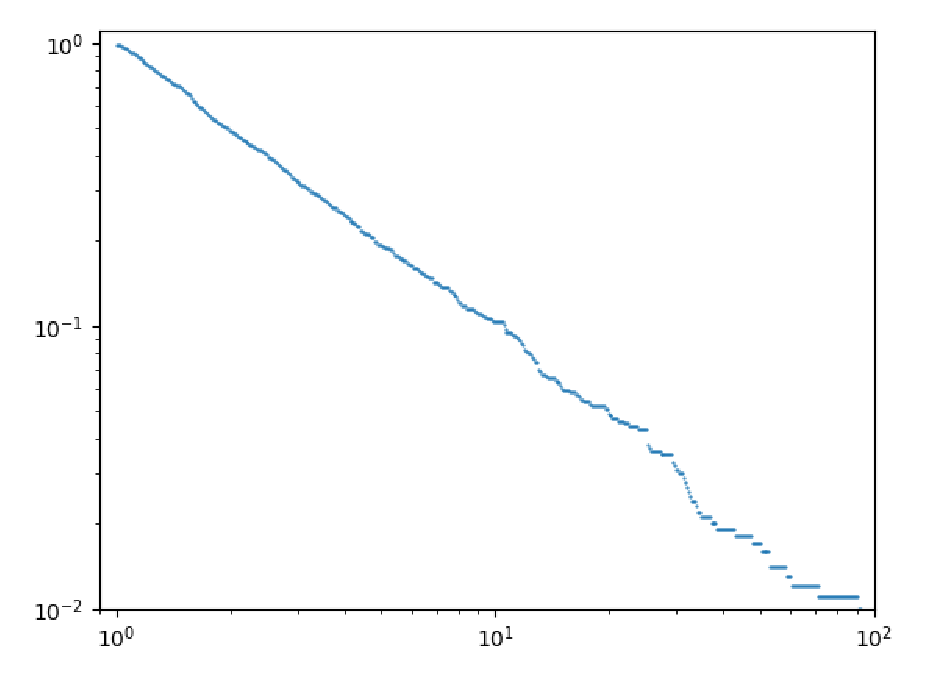
\includegraphics[scale=0.45]{colado11}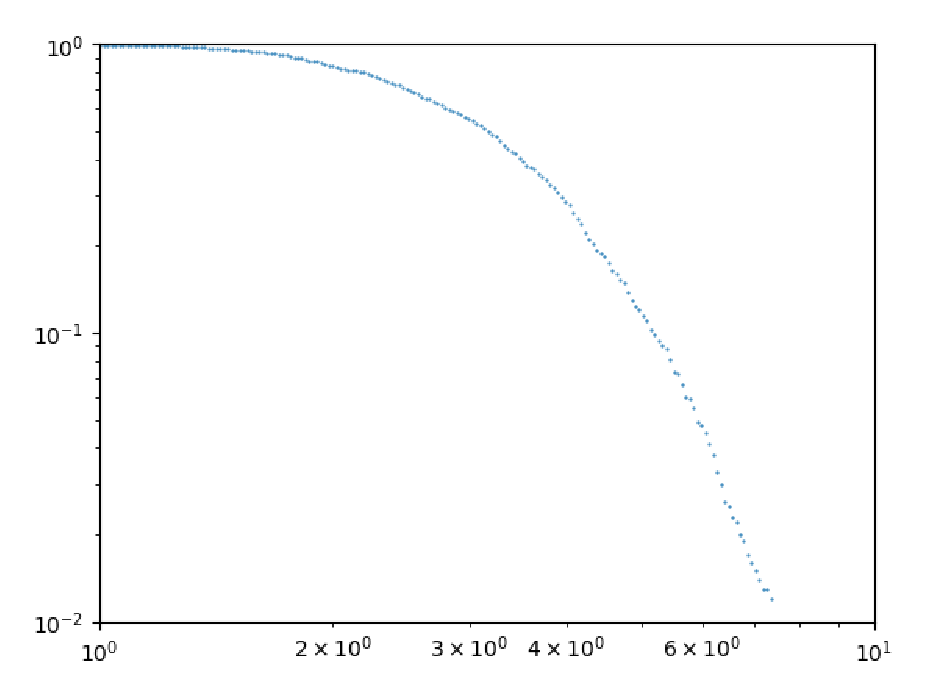
\includegraphics[scale=0.45]{colado12}\caption{{À esquerda temos a distribuição de $\left\langle m_{i}\right\rangle $ dos agentes, e a direita a distribuição $m_{0}\left(t\right)$ (isto é, o dinheiro do agente $i=0$) ao longo do período observado.}}
\end{figure}

Além disso, observando a distribuição agregada de riqueza do sistema, isto é, coletando a riqueza $m_{i}$ de todos os agentes ao final de cada passo da dinâmica, observamos um comportamento compatível com uma distribuição tipo-Gamma no corpo da distribuição, acompanhado de uma cauda mais pesada para grandes valores de riqueza. Embora a presença de uma lei de potência não seja conclusiva, o comportamento da cauda sugere um possível desvio em relação ao decaimento exponencial simples.

\begin{figure}[h!]
\centering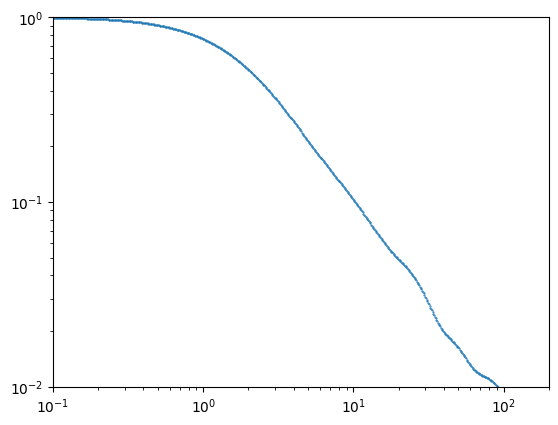
\includegraphics[scale=0.6]{colado13}
\end{figure}


Por fim, retornando o modelo com $\epsilon\left(t\right)=\alpha_{i}(t)\sum_{j}(1-\lambda_{j})m_{j}(t)$ realizamos um teste simples sorteando cada $\lambda_{i}$ de uma distribuiçao uniforme entre $0$ e $1$. Processo análogo para $\alpha_{i}$, com o adicional que normalizamos para que $\sum\alpha_{i}=1$. Dessa forma rodando uma simulação com $N=1000$, com $10000$ passos, considerando que avançamos um passo cada vez que atualizamos $m_{i}$ de todos agentes, coletamos $\epsilon_{i}\left(t\right)$ dos últimos $100$ passos (como são $1000$ agentes temos então $M=1000\times100=100.000$ dados). Utilizando intervalos de $\sqrt{M}$ dados obtemos então através do teste ``Ljung-Box'' que não há correlação. Além disso, calculando a média e desvio padrão de cada um dos intervalos, quando analisamos todos esses dados obtemos:

\[
\frac{\sigma_{media}}{\mu_{media}}=0.031\quad\frac{\sigma_{desvio}}{\mu_{desvio}}=0.030
\]

Portanto, neste cenário em específico, temos um indício que podemos aproximar $\epsilon\left(t\right)$ de fato a um ruído branco, porém nem todos os cenários foram explorados.

\subsection{Conclusão}

Os resultados obtidos ao longo deste trabalho permitem algumas conclusões importantes, ainda que nem todos os cenários possíveis tenham sido explorados. A discussão desenvolvida mostra certas dificuldades conceituais presentes nas tentativas de fundamentar modelos de econofísica a partir de hipóteses marginalistas, especialmente quando se procura incorporar elementos relacionados à produção, poupança, juros e circulação monetária sem introduzir mecanismos mais centrais da dinâmica capitalista, como lucro, acumulação de capital, concorrência efetiva ou a propriedade privada dos meios de produção. Nessas condições, a produção passa a funcionar essencialmente como um mecanismo formal de conversão entre dinheiro e mercadorias, permanecendo ausentes justamente os elementos que caracterizam a dinâmica do capitalismo enquanto sistema econômico. A introdução da esfera produtiva acaba então limitada a uma formalização parcial e insuficiente.

No primeiro modelo analisado, observamos que a introdução de funções utilidade do tipo Cobb-Douglas e mecanismos de otimização sob restrições orçamentárias conduz, após sucessivas simplificações, aos modelos cinéticos clássicos de troca monetária. O que ocorre, portanto, é menos uma eliminação da aleatoriedade do modelo e mais um deslocamento de sua origem formal. A aleatoriedade deixa de aparecer explicitamente como decorrente direta da transferência de riqueza e passa a ser localizada nas próprias preferências dos agentes, preferências essas cujos parâmetros passam a variar aleatoriamente a cada interação. Entretanto, após sucessivas reformulações microeconômicas, a dinâmica efetiva do sistema continua sendo essencialmente determinada por variáveis estocásticas de redistribuição monetária e, matematicamente, a aleatoriedade reaparece regulando diretamente a transferência de riqueza entre os agentes. Assim sendo mais do que uma abordagem marginalista da econofisica, o que temos é utilização de algumas formulações matemáticas para reescrever a aleatoriedade da transferência de riqueza como uma aleatoriedade no interesse do agente $i$ no que o agente $j$ tem a oferecer na troca.

Já no modelo generalizado, precisamos chamar a atenção para um processo semelhante. Apesar de partirmos novamente de funções utilidade do tipo Cobb-Douglas e mecanismos de otimização e considerações econômicas (omitindo novamente elementos cenrais) de equilíbrio perfeito, em um dado momento a fração $\alpha_{i}\left(t\right)$ da produção social total apropriada por cada agente é assumida ser arbitrária. Isso reconduz novamente a uma dinâmica de redistribuição de riqueza que tem como mecanismo principal a aleatoriedade. Se o objetivo do modelo é fundamentar a distribuição de riqueza a partir de uma abordagem marginalista, então a fração da produção social apropriada por cada agente não pode permanecer como um coeficiente essencialmente arbitrário.

Observamos então uma tensão metodológica importante: embora os modelos partam inicialmente de hipóteses econômicas relativamente estruturadas, uma parcela crescente da dinâmica passa progressivamente a ser determinada pelas propriedades estatísticas das variáveis aleatórias introduzidas. Em última instância, aspectos centrais da dinâmica econômica são ignorados desde o começo ou acabam substituídos por processos estocásticos sem uma devida justificação.

Isso não implica que os modelos de econofísica sejam inúteis ou incorretos. Pelo contrário, os resultados obtidos mostram que tais modelos são capazes de reproduzir qualitativamente distribuições de riqueza compatíveis com diversos padrões observados empiricamente, incluindo distribuições tipo-Gamma e caudas pesadas compatíveis com leis de potência em determinados regimes. Entretanto, os resultados sugerem que o corpo teórico mais adequado para fundamentar e interpretar esses modelos talvez esteja fora da abordagem marginalista.

A abordagem marxista, por exemplo, ao considerar que o elemento central do capitalismo reside nas relações sociais de produção, e não apenas em aspectos técnicos da circulação ou da troca, talvez apresente maior compatibilidade com modelos altamente abstratos de redistribuição monetária. Mesmo quando introdudzido uma abordagem probabilística da economia, os autores buscam justificá-las.

Nesse sentido, pode ser metodologicamente mais consistente abstrair completamente a esfera produtiva do que introduzir parcialmente seus elementos deixando de fora precisamente os mecanismos centrais da dinâmica de acumulação capitalista.

Assim, a principal limitação identificada neste trabalho não parece residir nos métodos estocásticos utilizados pela econofísica em si, mas na tentativa de conciliá-los com uma fundamentação microeconômica marginalista baseada em hipóteses de equilíbrio perfeito, agentes estruturalmente simétricos e ausência de mecanismos centrais da dinâmica capitalista.
\end{document}
